%%%%%%%%%%%%%%%%%%%%%%%%%%%%%%%%%%%%%%%%%%%%%%%%%%%%%%%%%%%%%%%%%%%%%%%%%%%%%%%%%%%%%%%%%%%%%%%%%%%%%%%%%%
\section{Introduction}\label{sec:introduction}

There are many works devoted to studying the nature of the Ethernet traffic\cite{selfsimilar-ethernet}. Classic Ethernet models used Poisson related processes. Initially, it makes sense since a Poisson-related process represents the probability of events occur in many independent sources with a known average rate, and independently of the last occurrence \cite{selfsimilar-ethernet} \cite{book-poisson}. But studies made by Leland et al.\cite{selfsimilar-ethernet} showed that the Ethernet traffic has a self-similar and fractal nature. Even if they can represent the randomness of an Ethernet traffic, simple Poisson processes can't express traffic "burstiness" in a long-term time scale, such as traffic "spikes" on long-range ripples. These characteristics are an indication of the fractal and self-similar nature of the traffic, that usually we express by distributions with infinite variance, called heavy-tailed. Heavy-tail means its distribution is not exponentially bounded\cite{sourcesonoff-paper}. Examples of heavy-tailed functions are Weibull, Pareto, Cauchy.  But heavy-tailed processes may guarantee self-similarity, but not necessarily they will ensure other important features like a high correlation between data and same mean packet rate.


Many investigations were made on the literature about the nature of the internet traffic\cite{selfsimilar-ethernet}\cite{analysis-self-similar}\cite{stochartic-selfsimilar}\cite{selfsimilar-highvariability}\cite{multi-player-online-game-self-similarity}, and many others on the modeling of stochastic functions for specific scenarios\cite{estimation-renewal-function-ethernet-traffic}\cite{modelling-of-self-similar}\cite{empirical-interarrival-study}\cite{modeling-concurrent-heavy-tailed}\cite{optimal-scheduling-of-heavy-tailed-traffic}\cite{modelling-of-self-similar}. But there are some limitations on this idea of finding a single model. Usually, not the same stochastic distribution will present a proper fitting for all possible kinds of traces\cite{sourcesonoff-paper}. Depending on some variables, such as the capture time, the number of packets or type of traffic, different functions may fit better the available data. On most of the works the best model representation for an Ethernet traffic is not chosen analytically but based on the researcher own data analyses and specific purposes\cite{hierarchical-dynamics-interarrival-times}\cite{modeling-concurrent-heavy-tailed}\cite{optimal-scheduling-of-heavy-tailed-traffic}. Also, some methods like linear regression may diverge sometimes. And it has already been demonstrated that a single model cannot represent arbitrary traffic traces\cite{sourcesonoff-paper}.  


In this work test the use of information criteria BIC(Bayesian information criterion) and AIC(Akaike information criterion) as tool for choosing the best fitting for inter-packet times of a traffic trace. It is an analytical method which spares and avoid human analyzes, is easy to be implemented by software, and don't relies on simulations and generation of random data. We fit a set of stochastic models through different methods and applying BIC and AIC to choose the best.  On this article, we analyze the results of inter-packet time fitting for one public available trace we call as \textit{skype-pcap}\footnote{It is a lightweight Skype capture, available at \href{https://wiki.wireshark.org/SampleCaptures}{https://wiki.wireshark.org/SampleCaptures}, named \textit{SkypeIRC.cap} }.


First, we explain the mathematical meaning of BIC and AIC and state the methods we are going to use to create a set of candidate models for our dataset. Then we define our cross-validation method based on a cost function $J$. Attributing weights from the best to the worst representation for each properties using randomly generated data with our stochastic fittings, we can choose the best possible traffic model among these fittings. We compare the results achieved by AIC/BIC and our cost function. We show that BIC and AIC are good at guessing the model with the lesser $J$ values. Also, we found that for traffic inter-packet times, that the difference between BIC and AIC values is minimal. So choosing one over the other do not seem to be a key question.  


%%%%%%%%%%%%%%%%%%%%%%%%%%%%%%%%%%%%%%%%%%%%%%%%%%%%%%%%%%%%%%%%%%%%%%%%%%%%%%%%%%%%%%%%%%%%%%%%%%%%%%%%%%
\section{AIC and BIC}\label{sec:aic-bic}

Suppose that we have an statistical model $M$ of some dataset ${\boldsymbol{x} = \{x_1, ..., x_n}\}$, with $n$ independent and identically distributed observations of a random variable $X$. This model can be expressed by a probability density function (PDF) $f(x| \boldsymbol{\theta})$, where $\boldsymbol{\theta}$ a vector of parameter of the PDF, $\boldsymbol{\theta} \in \mathbb{R}^{k}$ ($k$ is the number of parameters). The  likelihood function  of this model $M$ is given by:
\begin{equation}
L(\boldsymbol{\theta}|\boldsymbol{x} ) =  f(x_1|\boldsymbol{\theta})\cdot...\cdot f(x_n|\boldsymbol{\theta}) = \prod_{i = 1}^{n}f(x_i|\boldsymbol{\theta})
\end{equation}
Now, suppose we are trying to estimate the best statistical model, from a set ${M_1, ..., M_n}$, each one whit an estimated vector of parameters  ${\boldsymbol{\hat{\theta_1}}}, ..., {\boldsymbol{\hat{\theta_n}}}$. $AIC$ and $BIC$ are defined by:
\begin{equation}
AIC = 2k - \ln(L(\boldsymbol{\hat{\theta}}|\boldsymbol{x}))
\end{equation}
\begin{equation}
BIC = k\ln(n) - \ln(L(\boldsymbol{\hat{\theta}}|\boldsymbol{x}))
\end{equation}
In both cases, the preferred model $M_i$, is the one with the smaller value of $AIC_i$ or $BIC_i$.

%%%%%%%%%%%%%%%%%%%%%%%%%%%%%%%%%%%%%%%%%%%%%%%%%%%%%%%%%%%%%%%%%%%%%%%%%%%%%%%%%%%%%%%%%%%%%%%%%%%%%%%%%%
\section{Methodology}

We collect inter-packet times from the traffic capture we call \textit{skype-pcap}. Then, we estimate a set of parameters for stochastic processes, using a set of different methodologies, including linear-regression, maximum likelihood, and direct estimation. We are modeling: 

\begin{itemize}
    \item Weibull distribution, using linear regression, through the Gradient descendent algorithm;
    \item Normal distribution, using direct estimation the mean and the standard deviation of the dataset;
    \item Exponential distribution, using linear regression, through the Gradient descendent algorithm. We refer to this distribution as Exponential(LR);
    \item Exponential distribution, using a direct estimation of the dataset mean. We refer to this distribution as Exponential(Me);
    \item Pareto distribution, using linear regression, through the Gradient descendent algorithm. We refer to this distribution as Pareto(LR);
    \item Pareto distribution, using the maximum likelihood method. We refer to this distribution as Pareto(MLH);
    \item Cauchy distribution, using linear regression, through the Gradient descendent algorithm;
\end{itemize}

\begin{table*}[t]
\centering
\caption{Results of our modeling and simulation methodology for the traffic trace \textit{skype-pcap}. The stochastic processes are ordered form the worst to the best fitting, according to AIC and BIC.}
\label{tab:skype-results}
\begin{tabular}{lcccc}
\hline
Function        & AIC         & BIC        & \multicolumn{2}{c}{Parameters}      \\ \hline
Weibull         & $-2293.8$   & $-2283.8$ & $\alpha:0.522$ & $\beta:0.097$  \\
Exponential(Me) & $-426.13$   & $-421.1$  & \multicolumn{2}{c}{$\lambda:3.319$}  \\
Exponential(LR) & $96.9$   & $101.8$  & \multicolumn{2}{c}{$\lambda:1.505$}         \\
Pareto(MLH)     & $361.9$   & $371.8$  & $\alpha:0.0747$ & $x_m:5e-8$       \\
Normal          & $2423.8$    & $2433.8$   & $\mu:0.301 $   & $\sigma:0.749$ \\
Pareto(LR)      & $6411.0$   & $6421.08$  & $\alpha:0.413$ & $x_m:5e-8$       \\
Cauchy          & $13464.6$    & $13474.5$   & $\gamma:0.000275$ & $x_0:0.219$    \\ \hline
\end{tabular}
\end{table*}

Then, from these parametrized models, we estimate which best represent our dataset, using AIC  and BIC criterion. These results were obtained using Octave language\footnote{ \href{https://www.gnu.org/software/octave/}{https://www.gnu.org/software/octave/}}, and the scripts are available at \cite{projeto-github} for reproduction purposes. To see if our criterion of parameter selection can find which is the best model according to traffic modeling standards on realism and benchmarking\cite{validate-trafficgen}, we define a validation methodology. We generate randomly generated a same sized dataset compared to the original, using our stochastic processes fittings.  Then we compare it with the original and synthetic sample, trough three different metrics, all with a confidence interval of 95\%:

\begin{itemize}
\item Correlation between the sample data and the estimated model (Pearson's product-moment coefficient);
\item Difference between the original and the synthetic Hurst exponent;
\item Difference between the original and the synthetic mean inter-packet time;
\end{itemize}

The Pearson's product-moment coefficient, or simply correlation coefficient,  is an expression of the linear dependence or association between two datasets. To estimate it, we use the Octave's function \texttt{corr()}. The Hurst exponent is meter self-similarity and indicates the fractal level of the inter-packet times.  To estimate this value we use the function \texttt{hurst()} from Octave, which uses rescaled range method. Finally, the mean is also relevant, since it will meters if the packet rate of the approximation and the original trace are close to each other. 

To quantitatively check if AIC and BIC are suitable criteria for model selection for inter-packet times, we define a cost function based on the correlation, Hurst exponent and mean. Being $Cr$ the vector of correlations of the models ordered from the greater to the smaller. Let's define the vectors $Me$ and $Hr$ as the absolute difference (modulus of the difference) between mean and hurt exponent of the estimated models and the original dataset.  We order both from the smaller to the greatest values. Letting $\phi(V, M)$ be an operator who gives the position of a model $M$ in a vector $V$, we define the cost function $J$ as:
%The Pearson's product-moment coefficient, or simply correlation coefficient,  is an expression of the dependence or association between two datasets. Its value goes from -1 to +1. +1 means a perfect direct linear correlation. -1 indicates perfect inverse linear correlation. 0 means no linear correlation. So, as close the result reach 1, more similar are the inter-packet times to the original values. To estimate it, we use the Octave's function \texttt{corr()}.
%The Hurst exponent is meter self-similarity and indicates the fractal level of the inter-packet times. As close the result is from the original, more similar is the fractal level of the estimated samples from the original. To estimate this value we use the function \texttt{hurst()} from Octave, which uses rescaled range method. Finally, the mean is also relevant, since it will meters if the packet per second rate of the trace and its approximation model are close related. 
%To quantitatively check   if AIC and BIC are good criteria for model selection for inter-packet times, we define a cost function based on the correlation, Hurst exponent and mean. We defined a cost function $J$, based on the randomly generated data values with our estimated stochastic process. Being $Cr$ the vector of correlations ordered from the greater to the smaller. Let $Me$ and $Hr$ defined by the absolute difference between mean and hurt exponent of the estimated values and the original dataset. Both are ordered from the smaller to the greatest values. Letting $\phi(V, M)$ be an operator who gives the position of a model $M$ in a vector $V$, we define the cost function $J$ as:
\begin{equation}
J(M) = \phi(Cr, M) + \phi(Me, M) + \phi(Hr, M)
\end{equation}
The smaller is the cost $J$, the best is the model. Then we compare the results achieved by AIC and BIC, and $J$.


%%%%%%%%%%%%%%%%%%%%%%%%%%%%%%%%%%%%%%%%%%%%%%%%%%%%%%%%%%%%%%%%%%%%%%%%%%%%%%%%%%%%%%%%%%%%%%%%%%%%%%%%%%
\section{Results}
\begin{figure}[t]
{\centering
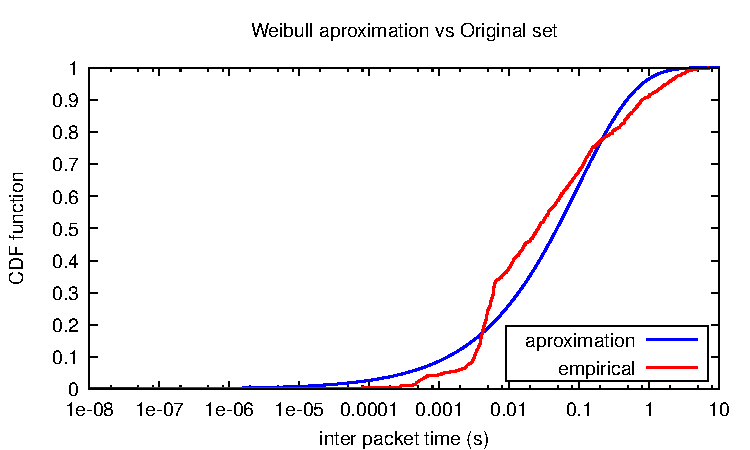
\includegraphics[width=\columnwidth]{figures/Weibull}
\caption{Cumulative distribution function(CDF) for Weibull fitting and empirical data for inter-packet times of \textit{skype-pcap}}
\label{fig:skype-weibull}\par}
\end{figure}
\begin{figure}[b]
{\centering
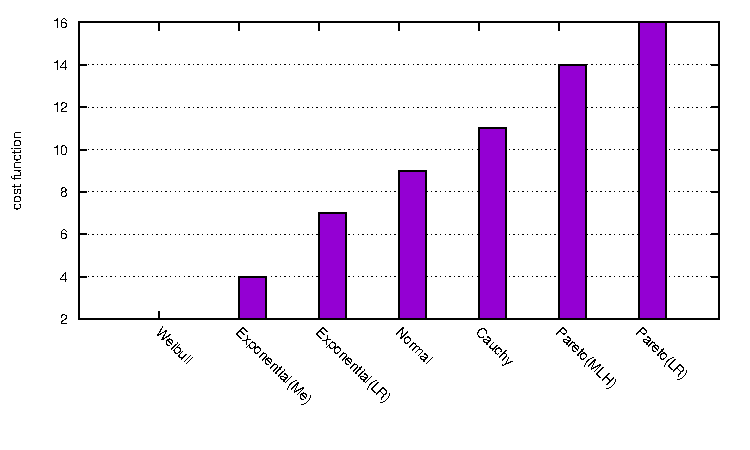
\includegraphics[width=\columnwidth]{figures/costFunction2}
\caption{Cost function $J$ of each stochastic process for \textit{skype-pcap}.}
\label{fig:cost-function}\par}
\end{figure}
In the table~\ref{tab:skype-results} we summarize our estimations for AIC, BIC, and the stochastic process estimated parameters. We organize the values in crescent order of quality, according to the selection criteria (the smaller, the better). In the figure ~\ref{fig:skype-weibull} we present the best fitting chosen both by BIC and AIC criteria. It is on log-scale, which provides a better visualization for small time values. Visually we can see that linear regression with Weibull distribution was able to provide a good approximation for this dataset.

The difference between BIC and AIC values in all simulations are much smaller than the difference between the distributions. This result indicates that for inter-packet times, using AIC or BIC to pick a model, do not influence the results significantly. According to BIC and AIC previsions, Weibull and Exponential (Me and LR) are the best options. Our cost functions points exact this order~\ref{fig:cost-function}. In fact, Weibull pointed as the best stochastic function by BIC and AIC, has half of the penalty imposed by the cost function $J$. The following model is not in the same order since some results are flipped. But still, no opposite correspondence is found. No result found by AIC and BIC were far from the one pointed by $J$. 


%\begin{figure}[h]
%{\centering
%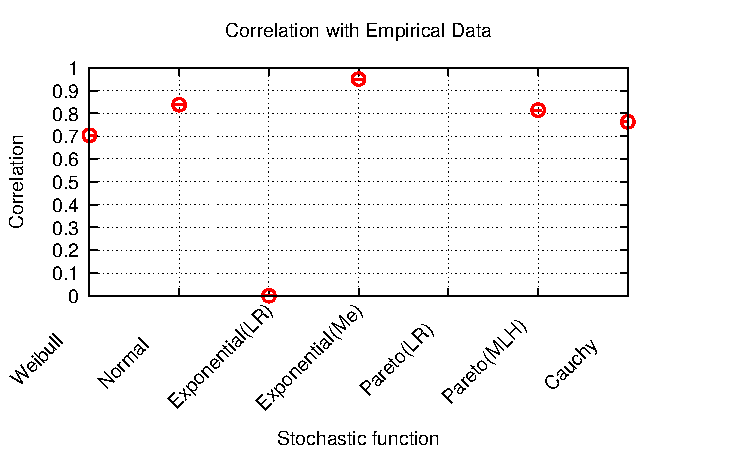
\includegraphics[width=\columnwidth]{figures/Correlation}
%\caption{Comparison between correlation of the used set of fittings, with a confidence of 95\%}
%\label{fig:skype-correlation}\par}
%\end{figure}


%\begin{figure}[t]
%{\centering
%\includegraphics[width=\columnwidth]{figures/HurstExponent}
%\caption{Comparison between the Hurst exponent of our approximated processes and the original data  with a confidence of 95\%}
%\label{fig:skype-hurst}\par}
%\end{figure}





%\begin{figure}[t]
%{\centering
%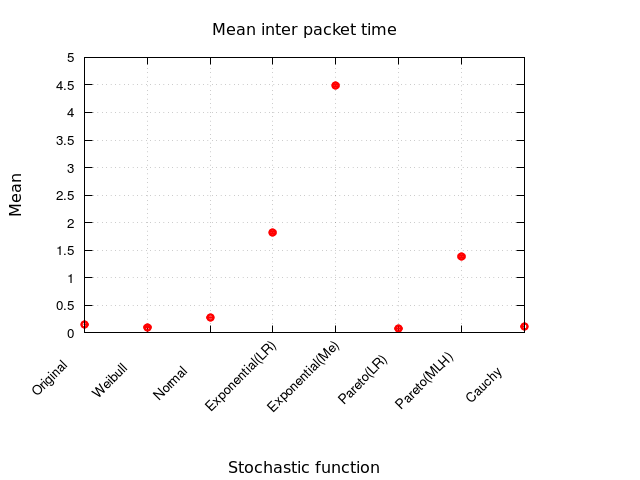
\includegraphics[width=\columnwidth]{figures/Mean}
%\caption{cap}
%\label{fig:skype-mean}\par}
%\end{figure}





%The difference between BIC and AIC values in all simulations are very small. Much smaller then the difference of these values between the distributions. This is an indication that for inter packet times, using AIC or BIC to pick a model, will not influence significantly the results. 

%According to BIC and AIC previsions, Weibull and Pareto(MLH and LR) are the best options. This was expected, since both are heavy-tailed functions. But Cauchy on most of the tests, even being a heavy-tailed distribution, seems to do no present a good fitting. This is effect of the fast divergence of tangent function, when we linearize our data. 

%From the figures ~\ref{fig:skype-correlation} and ~\ref{fig:fig:skype-hurst} we see that in therms of Correlation and Self-similarity it picket clearly the most related model: Weibull. Also in therms of mean packet rate it is still a good choice (along with Exponential(Me), Pareto(LR) and Cauchy). The third and the fourth choices (Pareto(LR)) and Exponential(Me) also are good options in most of these metrics. But, Pareto(MLH) is presented as the second best choice, and it had poor results in comparison to the others, especially on mean and correlation. This is the only model presented as good

%All these results are abstracted by the cost function $J$. As we can see, on all pcaps, the best function selected by BIC and AIC~\ref{tab:prototype-results} also had the small cost~\ref{fig:cost-function}. 

%Another important observation is the fact that exponential function was able to provide the best fitting for the \textit{wan-pcap}. The reasons for this behavior are both result of a much intense traffic with no long-range gaps, and the precision of the measurement.




\section{Conclusion}

In this work, we analyze how BIC and AIC perform being used as analytical selection criteria form stochastic models for Ethernet inter-packet times. Using a cross-validation methodology based on the generation of random data with these models, and pointing a cost function. We saw that both AIC or BIC and the cost function were able to pick the first models in the same order. Therefore, analytically with BIC and AIC, we were able to achieve the same results as pointed by our simulations. Even if AIC and BIC mathematical definitions are unaware of the specific requirements of Ethernet traffic modeling, such as same fractal-level and close packet per second rate, they still can point the best choices according to these constraints. 

Here in this work, we analyze just inter-packet times of a single trace. But at \cite{projeto-github} we perform the same methodology on different types of traffic captures, finding similar results. Therefore we can conclude that BIC and AIC are healthy alternatives for model selection of Ethernet inter-packet times models, and we can be safely them. Finally, we must point some advantages of BIC and AIC instead of simulations. Since it is an analytical model, no generation of random data is necessary,  being computationally cheaper and easy to code. Also, since we do not use a single stochastic function and parameterization strategy, it is resilient to the fact that some methods like liner-regression over Weibull may diverge sometimes. If it happens, BIC or AIC will discard this guesses, and choose another automatically.

%Also, except by the Pareto function modeled using the Maximum likelihood method, have comparative results between the simulations and the AIC/BIC goes. The best fittings according to the AIC/BIC usually returned very accurate models, with a small error between the mean and fractal level, and correlation close to one. The models selected as the worsts usually returned poor results.

%Also, it is important to notice that in some cases, some stochastic functions may perform poorly, and in other provide an accurate fitting, what justify the application of the criteria in all new experiments. For example, Weibull usually performs pretty well, but in some cases, perform poorly, and in others may even diverge. 

%We do not rely on only one type of parameterization. This turns our methodology more robust, since a linear regression may diverge. But always there will be a peaceable model, since our estimations for Normal, Exponential (Me) and Pareto (MLH) cannot. Models which the linear regression diverges, will have very high and positive BIC/AIC estimations, and will not stand as primary options.




















